\documentclass[FM,BP]{tulthesis}
\usepackage[czech]{babel}
\usepackage[utf8]{inputenc}
\usepackage[a-1a]{pdfx}
\usepackage{hyperref}
\usepackage{amsmath}
\usepackage{amssymb}
%\DeclareTextSymbolDefault{\S}{T1}
\newcounter{Vzorce}
\addtocounter{Vzorce}{1}

\TULtitle{Řešení optimalizační úlohy LASSO pomocí proximálních algoritmů}{Solution to LASSO Using Proximal Algorithms}
\TULprogramme{B2646}{Informační technologie}{Information Technology}
\TULbranch{1802R007}{Informační technologie}{Information Technology}
\TULauthor{Václav Langr}
\TULsupervisor{doc. Ing. Zbyněk Koldovský, Ph.D.}

\begin{document}
\ThesisStart{male}{zadan}
\begin{acknowledgement}
Chtěl bych tímto poděkovat všem, kteří mne podporovali. Především mé rodině za velikou podporu, díky které mi bylo umožněno studovat. 


Zároveň bych chtěl poděkovat také vedoucímu této práce doc. Ing. Zbyňku Koldovskému, Ph.D. za velice přínosné konzultace, rady a trpělivost.
\end{acknowledgement}
\clearpage
\begin{abstractCZ}
Tato bakalářská práce je zaměřena na rekonstrukci řídkého vektoru z jeho komprimovaného pozorování. Pro rekonstrukci se využívá optimalizačního problému LASSO a jeho řešení pomocí proximálních algoritmů. Po vytvoření takového algoritmu, který je schopen původní signál rekonstruovat, se využívá metody Monte Carlo pro simulaci algoritmu na větším souboru dat. Pro takto získaný výpočet je zjištěna kvadratická chyba řešení LASSO od původního vektoru dat, která je následně porovnávána s teoretickou chybou.


Vypracování této bakalářské práce bylo rozděleno do několika navazujících částí. Prvním a také nejdůležitějším krokem bylo nastudování vlastností proximálních algoritmů a výpočet proximálního operátora při různých vstupních funkcích. Po takto provedené rešerši proximálních algoritmů proběhla také rešerše vlastností optimalizační úlohy LASSO. Následně bylo možné přistoupit k implementaci algoritmu v programovacím jazyce a vývojovém prostředí MATLAB. Při postupné implementaci byl algoritmus upraven tak, aby vždy dokonvergoval ke správnému nebo alespoň přibližnému řešení optimalizačního problému. Z tohoto důvodu byl algoritmus rozšířen o podmínky optimality, jež ukončují výpočet při dosažení poměrně přesné aproximace. Dále byl rozšířen o výpočet dynamické velikosti kroku. S takto připraveným algoritmem mohla být vytvořena metoda Monte Carlo, která generuje nekomprimovaný řídký vektor dat, měřící matice, jejichž prvky mají Gaussovo rozložení, a parametr lambda v zadaném rozsahu s logaritmickým rozdělením.  


Výsledek této práce může být využit pro další zpracování. Jedním z možných použití je např. pro vytvoření nového datového formátu, ve kterém by byl uložen jen komprimovaný vektor dat případně i měřící matice, pokud by nebyla shodná pro všechny komprimace. Na straně klienta by byl tedy pouze zrekonstruován původní nekomprimovaný signál.


\textbf{Klíčová slova:} MATLAB, proximální algoritmus, proximální operátor, LASSO, Monte Carlo
\end{abstractCZ}
\vspace{2cm}
\begin{abstractEN}
This bachelor thesis is focused on reconstruction of sparse vector from his compressed observation. For the reconstruction is used the LASSO problem and its solution using proximal algorithms. After creation of an algorithm that is able to restore the original signal is used Monte Carlo method for simulation of the algorithm with bigger set of data. Then is calculated the squared error for the found solution and the original data that is compared with the theoretical error.


Realization of this bachelor thesis was divided into several parts. The very first and the most important step was studying the properties of proximal algorithms and evaluation of proximal operator for different functions. After the research on proximal algorithms there was also research on the properties of the LASSO. After that is was possible to implement algorithm using MATLAB language and development environment. The algorithm was modified during the implementation so it always converges into correct or at least approximate solution of LASSO. Due to this reason optimality conditions were added that terminates solving if the approximation is very accurate and a computation of dynamical step size. This prepared algorithm could be used for creation of Monte Carlo method that generates uncompressed sparse vector of data, random measurement matrix with Gaussian distribution and a lambda parameter within an interval with logarithmic distribution.


The result of this thesis can be used for another usage. One of the possible usage is for example creation of a new data format. The compressed data would be saved in this format and only if the measurement matrix is not the same for all compressions it would be also saved. On the client side the original uncompressed signal would be recovered.


\textbf{Keywords:} MATLAB, Proximal Algorithm, Proximal Operator, LASSO, Monte Carlo
\end{abstractEN}
\clearpage
\tableofcontents
\listoffigures
\listoftables
\pagebreak

\renewcommand{\baselinestretch}{1.5}
\setlength\parindent{1.2cm}
\selectfont

\chapter{Úvod}
\label{ch:uvod}
V dnešním světě, kdy získáváme stále více důležitých a velkých dat je stále důležitější nějakým způsobem získaná data komprimovat. Z tohoto důvodu se tato práce zabývá komprimací dat a následnou rekonstrukcí u koncového uživatele. Bude pro to použito nového přístupu pomocí proximálních algoritmů, které jsou rychlé a jednoduché na implementaci.

Základní měření odpovídá funkci, viz \ref{eq:Zakladni mereni}, kde jsou původní data $x_0 \in \mathbb{C}^n$ transformovány měřící maticí $A \in \mathbb{C} ^{m \times n}$, kde $m$ je počet řádků a $n$ počet sloupců matice a v poslední řadě je nutné uvažovat i náhodná data $z \in \mathbb{C}^m$, v našem případě toto reprezentuje náhodný šum. Takto jsou získaná nová data $y \in \mathbb{C}^m$. V obecných případech platí, že $m \geq n$, ale takto nedochází k žádné komprimaci dat případně by i vzrostl počet dat. Následná rekonstrukce by se tak redukovala pouze na spočtení inverzní, v případě obdélníkové matice pseudoinverzní, matice $A^{-1}$ a spočtení původních dat $x_0$. Tato bakalářská práce se zabývá případy, kdy $m < n$ a nelze tedy použít pseudoinverzní matici.

\begin{equation} \label{eq:Zakladni mereni} \tag{Vzorec \theVzorce}
y = A \times x_0 + z
\end{equation}
\stepcounter{Vzorce}

Dle pravidel lineární algebry tak existuje nekonečně mnoho řešení a je tak nemožné v tomto případě zrekonstruovat původní data. Nicméně ve skutečnosti lze data zrekonstruovat a to za podmínky, že původní vektor dat $x_0$ je řídký, tedy většina prvků z $x_0$ je rovno $0$. Právě z tohoto důvodu jsou kompresní algoritmy, například pro kompresi formátu JPEG, kdy se ukládají pouze největší koeficienty diskrétní kosinové transformace, tak efektivní. Toto ale není jedinná podmínka, nutná k úspěšné rekonstrukci. Další podmínkou je správná volba měřící matice $A$. Například, při volbě diagonální jednotkové matice, by komprimovaná data $y$ byla z velké části nulová. Z tohoto důvodu by pak bylo nemožné rekonstruovat původní data. Jelikož je toto téma velice zkoumané v dnešní době, vzniklo mnoho výzkumů, které se problematikou tohoto problému zabývají velice podrobně. Právě tyto výzkumy ukazují, že aby došlo k jisté rekonstrukci, je potřeba využít měřící matice o náhodných prvcích z normovaného normálního rozdělení, tj. normální rozdělení s nulovou střední hodnoutou a jednotkovým rozptylem.

\chapter{Optimalizační problémy}
\label{ch:optproblem}
Optimalizační problém je takový problém, kdy hledáme nejlepší možné řešení $x$ ze všech možných a to tak, aby $f(x)$ bylo maximální nebo minimální, podle zadané úlohy. Hledáme tedy globální maximum, respektive minimum, funkce, kterou se snažíme vyřešit. 


Veškeré další řešení je založeno na tom, že je lze zapsat v neomezeném tvaru. V tomto tvaru se minimalizuje obecný vstup $x$ přes součet $m$ konvexních funkcích $f_0 \ldots f_m$, které náleží množině $\mathbb{R}^n$. Takto zapsaný problém by byl definován jako:
\begin{equation} \label{eq:Obecny problem} \tag{Vzorec \theVzorce}
\underset{x \in \mathbb{R}^n} {\mathrm{min}} f_{0}(x)+\ldots+f_{m}(x)
\end{equation}
\stepcounter{Vzorce}

Nicméně, jelikož lze uvažovat jakoukoliv výše zmíněnou funkci, naskýtá se tu typický problém. Některé funkce nejsou diferenciovatelné. Z tohoto důvodu se nadále bude na funkce a jejich řešení nahlížet jako na samostatný problém.

\section{Optimalizační problém LASSO}
Problém rekonstrukce původních dat se vyskytuje v nejrůznějších oborech. Mezi tyto obory patří strojové učení, zpracování signálů a další. Jeden z možných přístupů je využít minimalizace a to ve tvaru, který popisuje \ref{eq:Obecne LASSO}. Funkce $f_1(x)$ ve vzorci je libovolná a volí se podle toho, jaké vlastnosti mají vstupní data. 

\begin{equation} \label{eq:Obecne LASSO} \tag{Vzorec \theVzorce}
\underset{x} {\mathrm{argmin}} ~\left\{\left\|y-A \times x\right\| ^2 _2+ \lambda \times f_1(x)\right\}
\end{equation}
\stepcounter{Vzorce}

V případě řídkého vektoru se volí funkce $\left\|x\right\|_1$ a vyniká tak vztah popsaný níže. Tento nový vztah zároveň řeší dva problémy a to rekonstrukci původních dat $x_0$ a jejich odšumnění.

\begin{equation} \label{eq:Konkretni LASSO} \tag{Vzorec \theVzorce}
\underset{x} {\mathrm{argmin}} ~\left\{\left\|y-A \times x\right\| ^2 _2+ \lambda \times \left\|x\right\|_1\right\}
\end{equation}
\stepcounter{Vzorce}

Jelikož obě funkce optimalizačního problému LASSO obsahují funkci $l$ normy, musí být zmíněna i její definice, která je popsána \ref{eq:norma}. V případě $l1$ normy tak vyniká pouze suma absolutních hodnot a vzniká tak další problém, jak bylo naznačeno v kapitole \ref{ch:optproblem}. Pro lepší ilustraci je tato funkce zobrazena v \ref{fig:abs}. Z tohoto zobrazení je patrné, že tato funkce má nekonečně mnoho derivací v bodě $[0,0]$ a nelze tak spočítat její derivaci, což je velice důležité pro pozdější zpracování.

\begin{equation} \label{eq:norma} \tag{Vzorec \theVzorce}
\left\|x\right\|_p = \left(\sum_{i=1}^{n} \left|x_i\right|^p\right)^{1/p}
\end{equation}
\stepcounter{Vzorce}

\begin{figure}[!ht]
\begin{center}
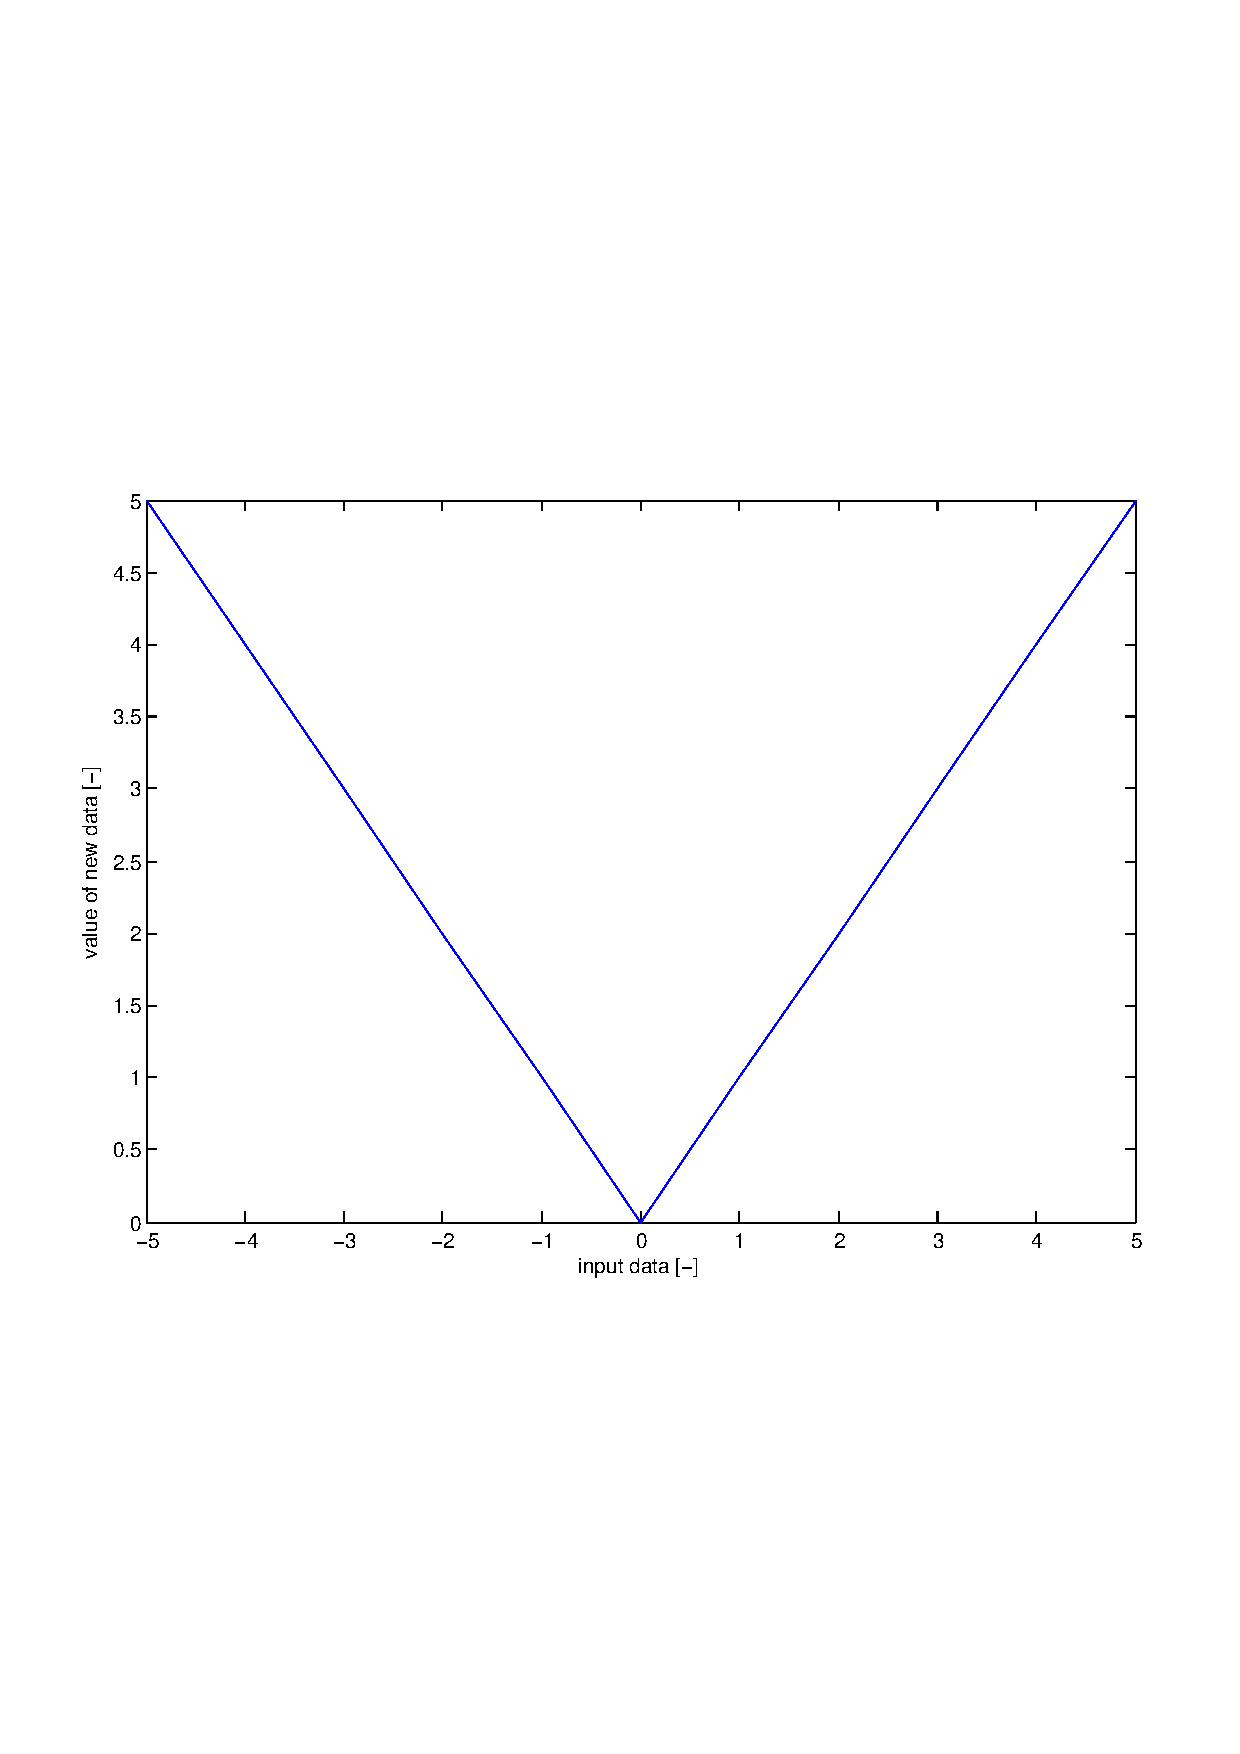
\includegraphics[scale=0.55]{obr/abs.pdf}
\end{center}
\caption{Graf $\left|x\right|$}
\label{fig:abs}
\end{figure}

\chapter{Proximální algoritmy}
\label{ch:proxalg}
Jednou z možností, jak vyřešit problém zmíněný v předchozí kapitole, je využít proximální algoritmy a proximální operátory příslušející zadaným funkcím. Proximimální algoritmus je:
\begin{equation} \label{eq:proxAlg} \tag{Vzorec \theVzorce}
x_{n+1} = prox_{\lambda \times f}(x_{n})
\end{equation}
\stepcounter{Vzorce}
V tomto vzorci je $f$ uzavřená konvexní funkce, která splňuje $f : \mathbb{R^{m}} \rightarrow \mathbb{R} \cup \left\{+\infty\right\}$. Jak je patrné, proximální algoritmy jsou velice výhodné, pouze pokud je výpočet proximálního operátora efektivní a velice rychlý na výpočet. Pokud by nebylo splněno toto kritérium, tak by se mnoho času strávilo vyhodnocováním proximálního operátoru, které se musí provádět v každé iteraci algoritmu. Zároveň proximální operátor zjednodušuje problém, který by jinak byl obtížně řešitelný. Další obrovskou výhodou těchto algoritmů je také fakt, že byly navrženy pro co nejobecnější využití a lze je tak využít v nejrůznějších problémech.

\section{Proximální operátor}
Jak již bylo naznačeno v kapitole \ref{ch:proxalg}, bude využito proximálního operátoru pro rekonstrukci dat. 

\begin{figure}[!ht]
\begin{center}
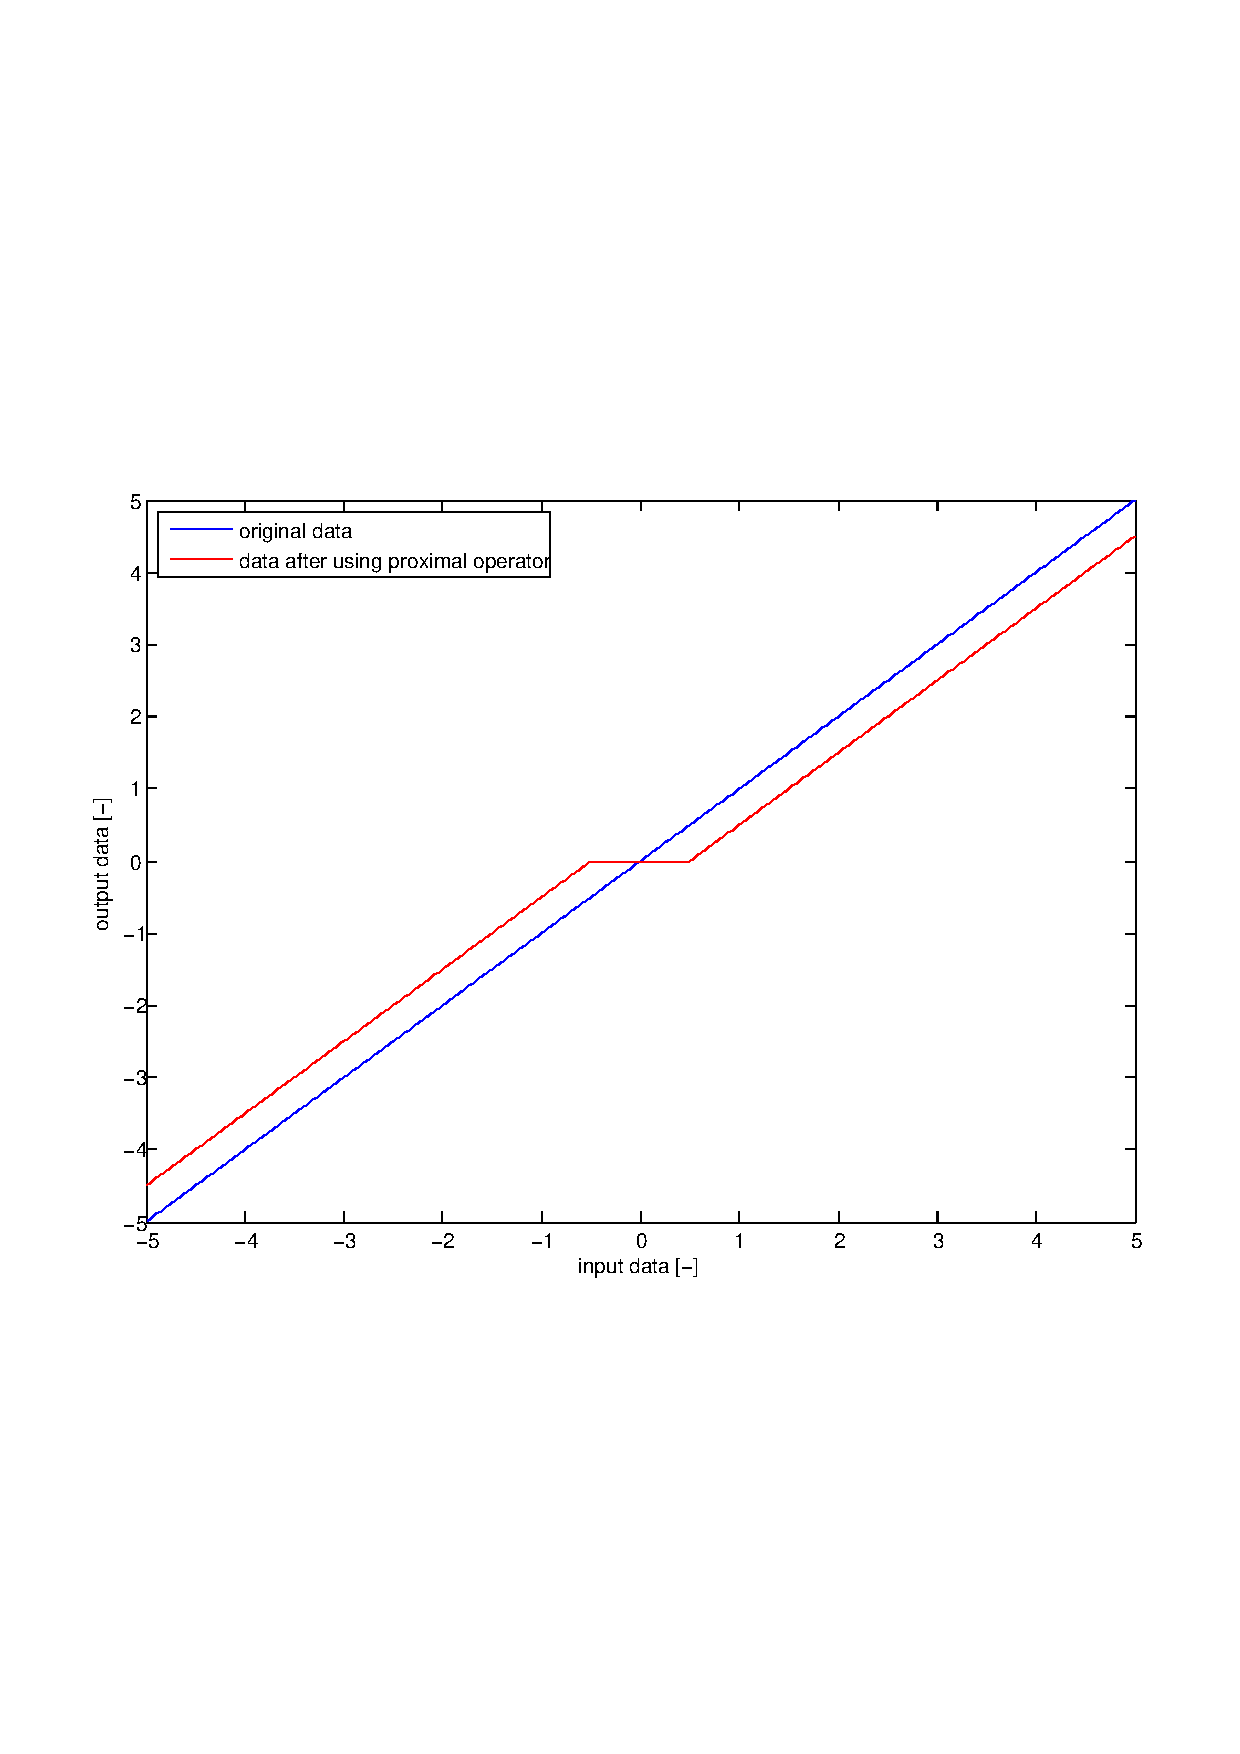
\includegraphics[scale=0.55]{obr/threshhold.pdf}
\end{center}
\caption{Průběh zvoleného proximálního operátoru pro $\lambda$ = 0.5}
\label{fig:threshhold}
\end{figure}

\chapter{Dopředno-zpětný algoritmus}
\label{ch:fwbw}
Jako hlavní algoritmus, na který se tato práce zaměřuje, je dopředo-zpětný algoritmus. Jeho základní varianta, popsaná obrázkem \ref{fig:fw-bw alg}, používá pevnou délku kroku. Je to iterační algoritmus, který získá na vstupu komprimovaná data $y$, měřící matici $A$, velikost kroku $\alpha$ a parametr $\lambda$, který si volí uživatel.
\begin{figure}[!ht]
\begin{center}
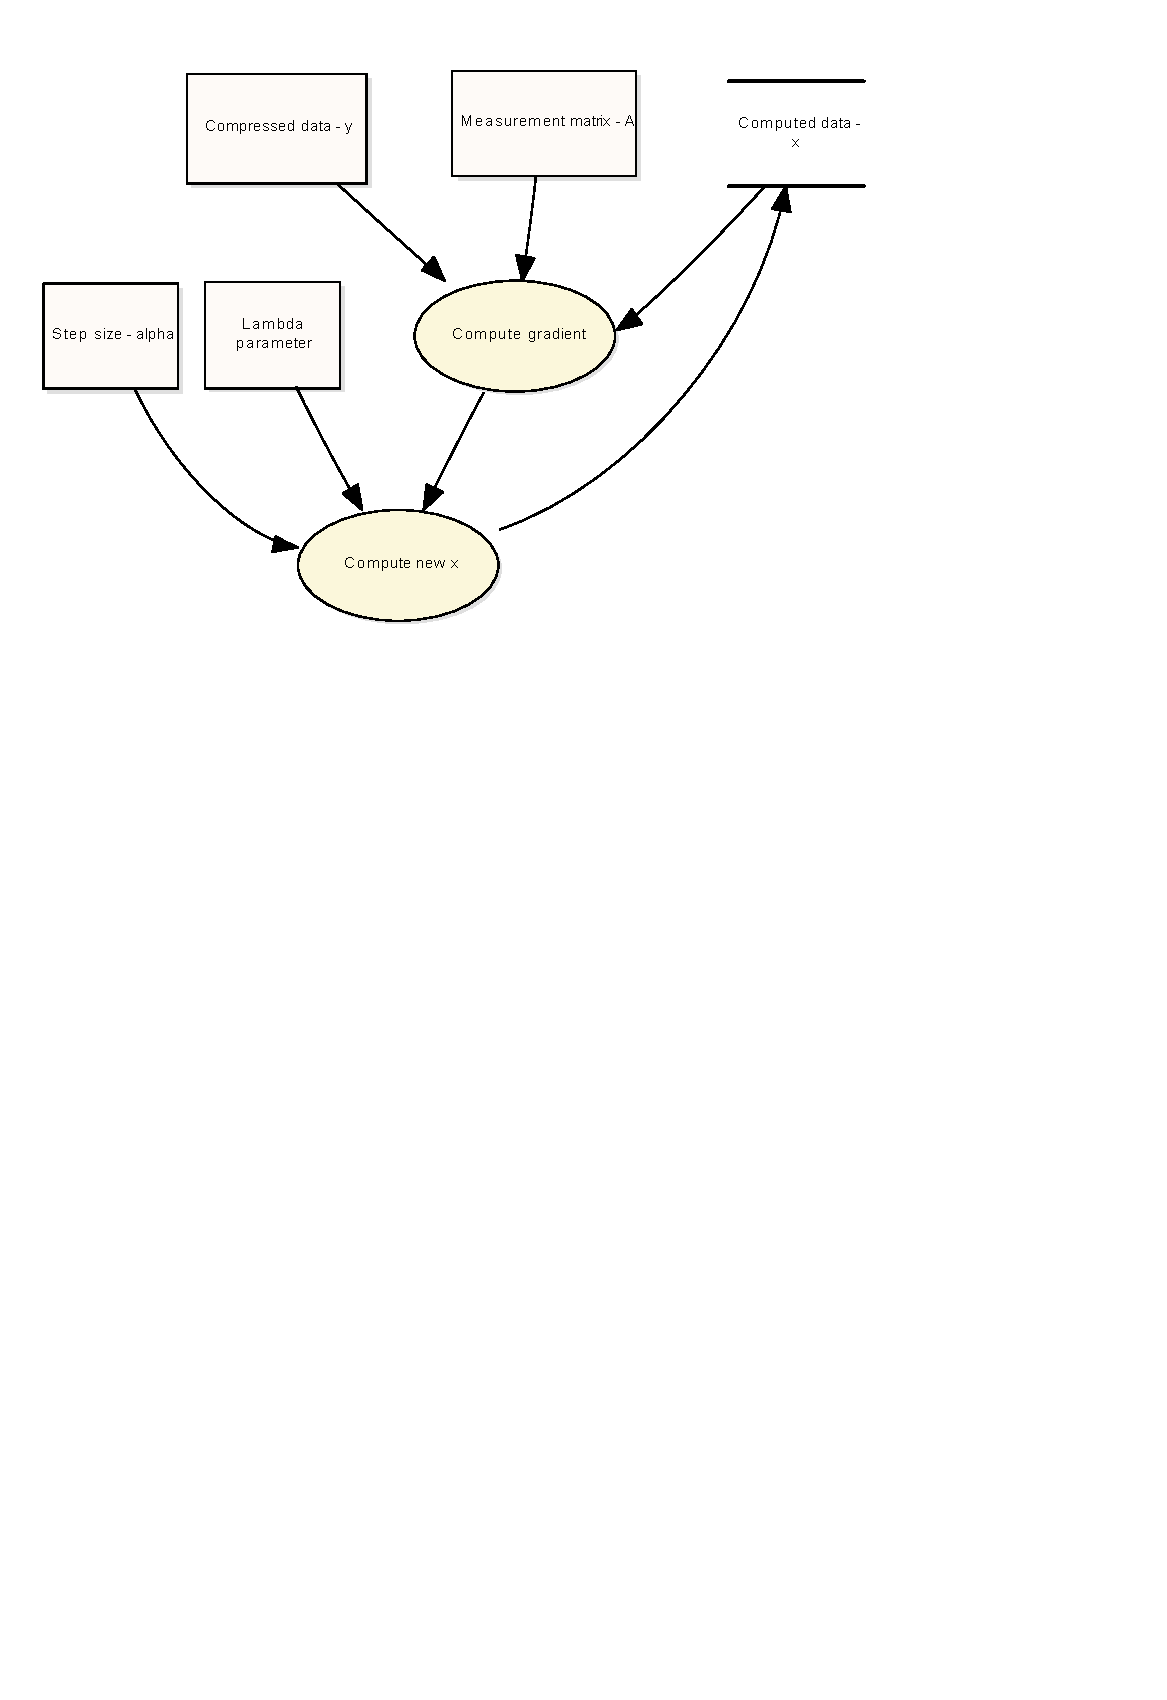
\includegraphics[scale=0.7]{obr/forwardbackward.pdf}
\end{center}
\caption{Schéma dopředno-zpětného algoritmu}
\label{fig:fw-bw alg}
\end{figure}

Za pomoci těchto údajů se v každém kroku počítá gradient diferenciovatelné části optimalizační úlohy LASSO, jehož předpis funkce je \ref{eg:Gradient LASSO}.
\begin{equation} \label{eg:Gradient LASSO}  \tag{Vzorec \theVzorce}
\partial f(x) = -2 \times A^T \times (y-A \times x)
\end{equation}
\stepcounter{Vzorce}
Poté se již spočítá nový vektor dat $x$ za pomoci proximálního operátoru, jehož průběh je znázorněn v \ref{fig:threshhold}, dle vzorce viz \ref{eg:ComputeX}. 
\begin{equation} \label{eg:ComputeX}  \tag{Vzorec \theVzorce}
x_{n+1} = prox_{\lambda \times \alpha _{n}}(x_{n}- \alpha _{n} \times \partial f(x_{n}))
\end{equation}
\stepcounter{Vzorce}

\section{Varianta s pevnou délkou kroku}

\begin{figure}[!ht]
\begin{center}
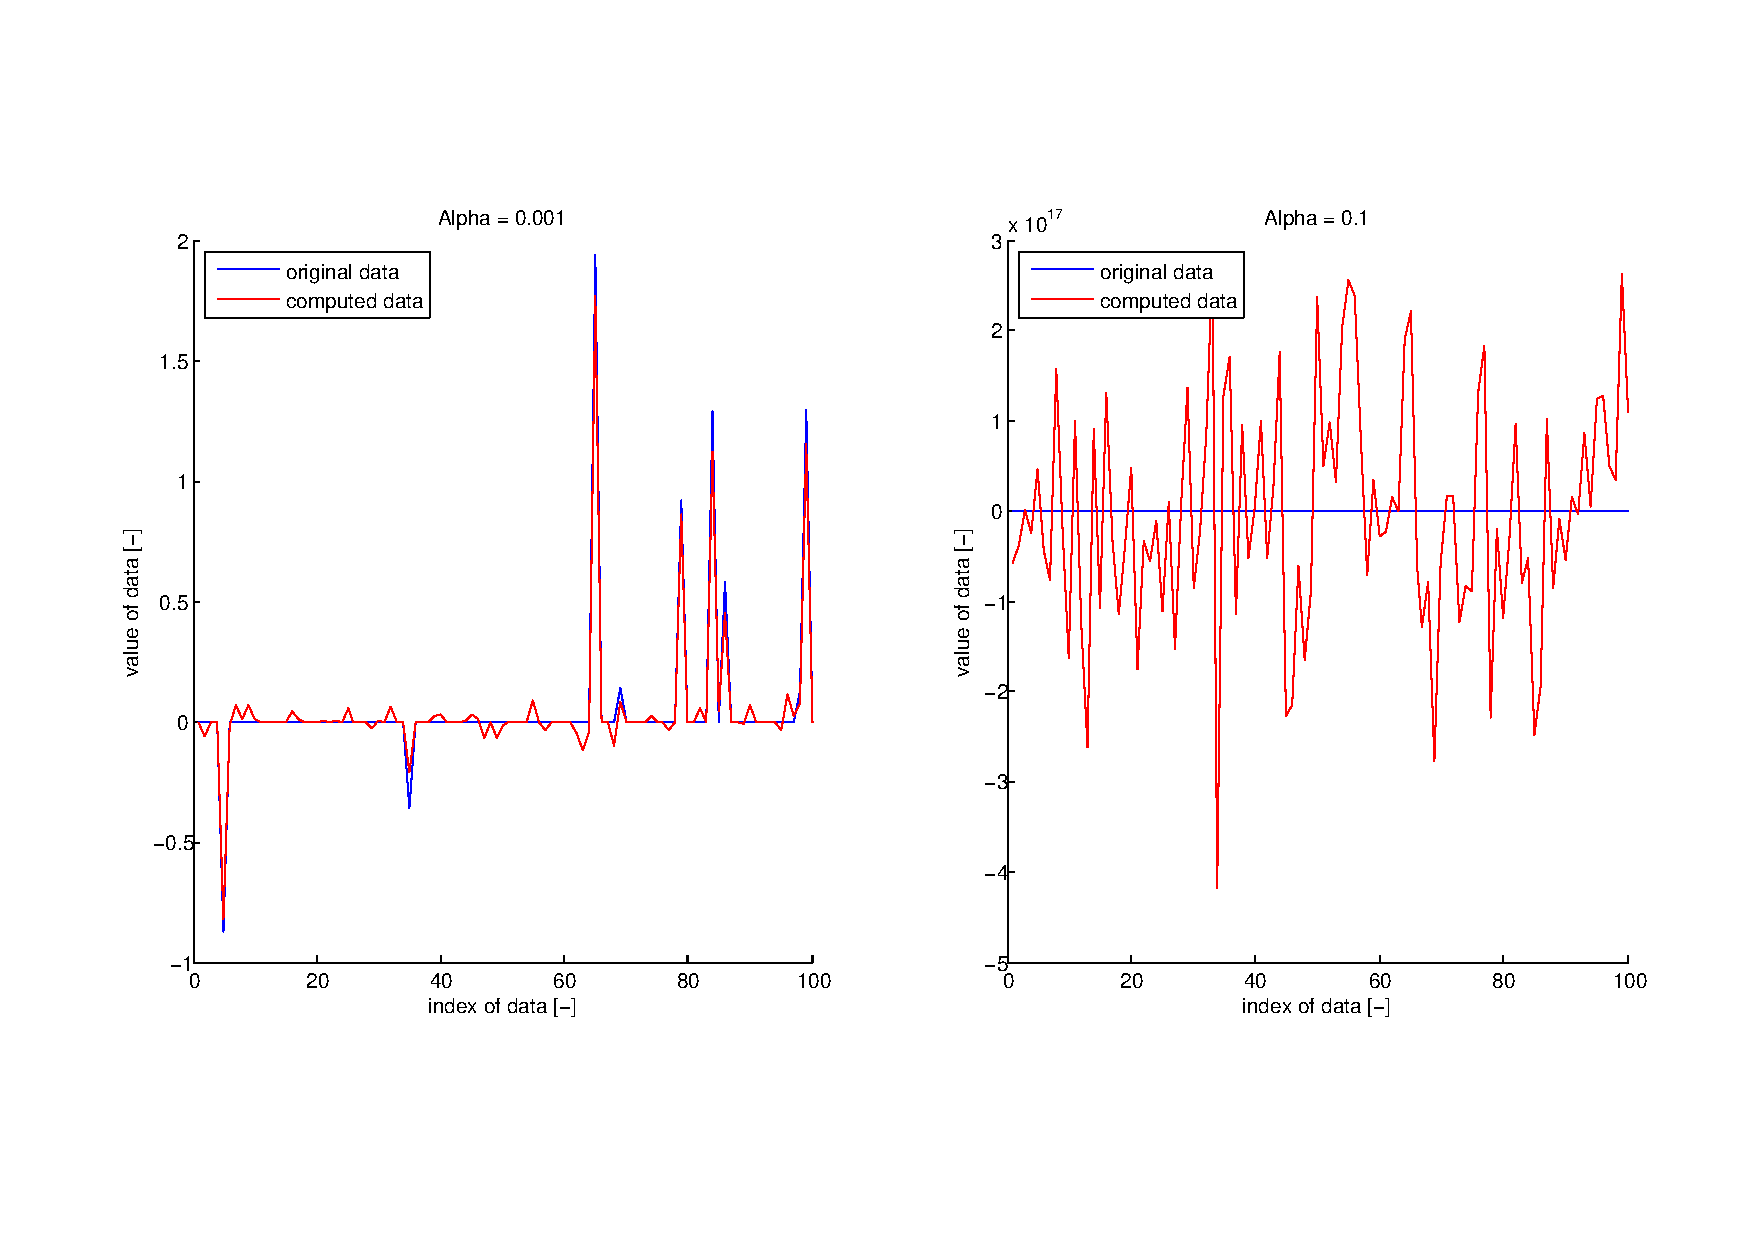
\includegraphics[scale=0.5]{obr/basic.pdf}
\end{center}
\caption{Ukázka průběhu algoritmu při různé volbě délky kroku}
\label{fig:basicAlpha}
\end{figure} 

\section{Dynamická délka kroku}
\begin{figure}[!ht]
\begin{center}
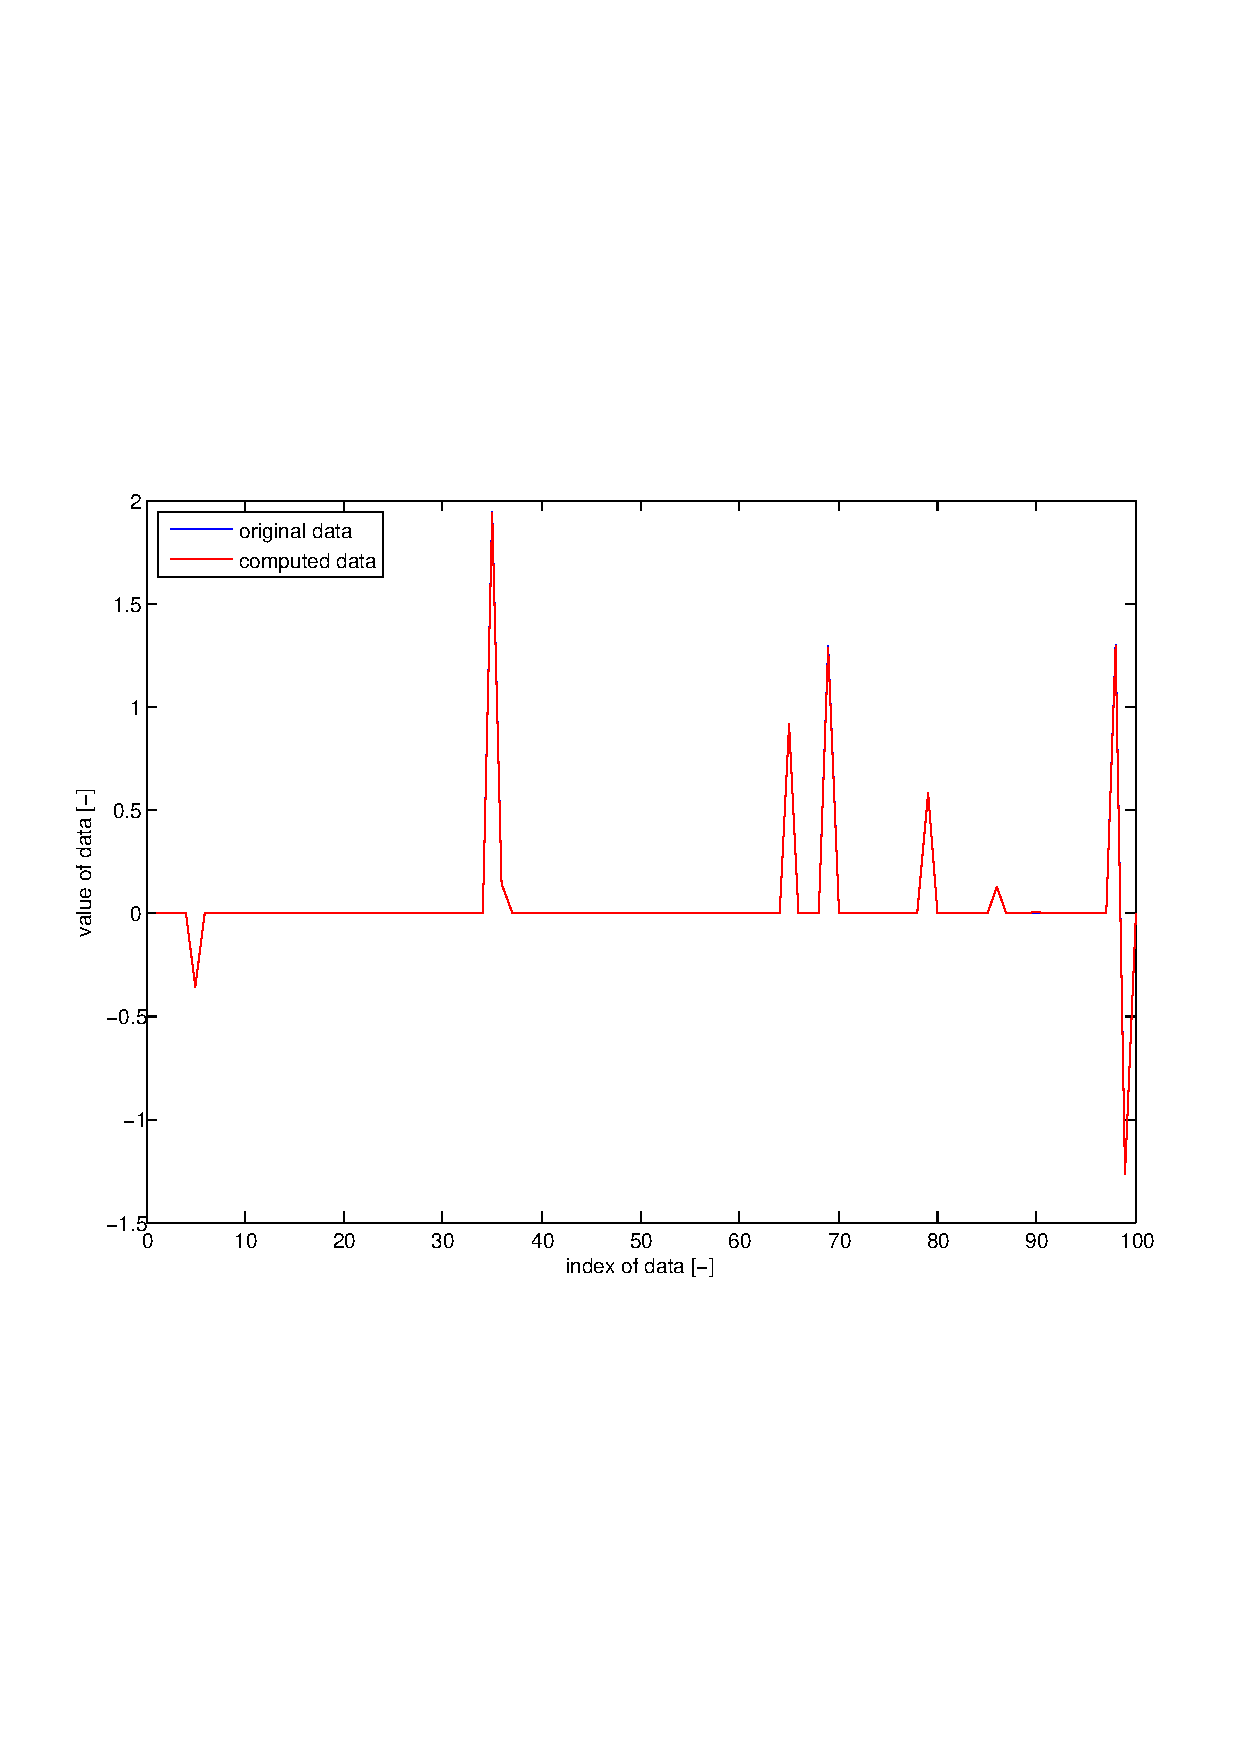
\includegraphics[scale=0.5]{obr/dynamic.pdf}
\end{center}
\caption{Ukázka průběhu algoritmu s dynamickou délkou kroku}
\label{fig:dynamicAlpha}
\end{figure}

\section{Podmínky optimality}

\section{Konečná verze algoritmu}

\chapter{Monte Carlo simulace}
\label{ch:simulace}
\section{Realizace simulace}
\section{Ukládání výsledků}
\section{Výsledky}

\chapter{Závěr}
\label{ch:end}

\renewcommand{\bibname}{Seznam použité literatury}
\begin{thebibliography}{99}
\bibitem{convexOptimization} BOYD, Stephen P a Lieven VANDENBERGHE. Convex optimization. Seventh printing with corrections. New York: Cambridge University Press, 2004. ISBN 05-218-3378-7.
\bibitem{homotopy}Z. Koldovský and P. Tichavský, "A Homotopy Recursive-in-Model-Order Algorithm for Weighted Lasso," Proc. of the 41st IEEE International Conference on Audio, Speech, and Signal Processing (ICASSP 2014), Florence, Italy, pp. 4151-4155, May 2014.
\end{thebibliography}
\end{document}
